\documentclass[10pt]{beamer}

\usepackage{color}
\usepackage{listings}

\usetheme{Hannover}
\usefonttheme{serif}
\usecolortheme{seagull}
\beamertemplatenavigationsymbolsempty
\setbeamertemplate{blocks}[rounded][shadow=false]
\setbeamertemplate{bibliography item}{\insertbiblabel}

\definecolor{Blue}{rgb}{0.0, 0.0, 0.8}
\definecolor{DarkGreen}{rgb}{0.0, 0.5, 0.0}
\definecolor{DarkGray}{rgb}{0.5, 0.5, 0.5}
\definecolor{Gray}{rgb}{0.8, 0.8, 0.8}
\definecolor{Orange}{rgb}{0.8, 0.5, 0.0}
\definecolor{White}{rgb}{1.0, 1.0, 1.0}

\lstset{
  basicstyle=\ttfamily\footnotesize,
  breakatwhitespace=false,
  breaklines=true,
  captionpos=b,
  commentstyle=\color{DarkGreen},
  escapeinside={\%*}{*)},
  extendedchars=true,
  frameshape={RYR}{Y}{Y}{RYR},
  keepspaces=true,
  keywordstyle=\color{Blue},
  numbers=left,
  numbersep=6pt,
  numberstyle=\tiny\color{DarkGray},
  rulecolor=\color{Gray},
  showspaces=false,
  showstringspaces=false,
  showtabs=false,
  stepnumber=1,
  stringstyle=\color{Orange},
  tabsize=2
}

\title{Who's Hacking Who?}
\subtitle{
  From Russia with Love
  \vspace{0.5cm}
  \\
  
\includegraphics[height=3cm,keepaspectratio]{hackers.jpg}
  \\
  \scriptsize{\emph{Hackers - 1995}}
}
\author[UH CSS]{D.~Barry\inst{1} \and L.Bol\inst{1}}
\institute{
  \inst{1}
  Computer Science Society
  \\
  University of Hertforshire
}
\date{October, 2016}
\subject{Computer Science}

\begin{document}
  %%%%%%%%%%%%%%%%%%%%%%%%%%%%%%%%%%%%%
  % Title
  %%%%%%%%%%%%%%%%%%%%%%%%%%%%%%%%%%%%%
  \frame{\titlepage}
  \begin{frame}
    \frametitle{Table of Contents}
    \begin{block}{}
      \vspace{0.5cm}
      \tableofcontents
      \vspace{0.5cm}
    \end{block}
  \end{frame}
  %%%%%%%%%%%%%%%%%%%%%%%%%%%%%%%%%%%%%
  % Introduction
  %%%%%%%%%%%%%%%%%%%%%%%%%%%%%%%%%%%%%
  \section[Intro]{Introduction}
  \begin{frame}
    \frametitle{Credentials}
    \centering
    \begin{tabular}{| r | c | c |}
      \hline
                 & Daniel Barry                                            & Lukasz Bol     \\
                 & 
\includegraphics[width=2cm,keepaspectratio]{dbarry.jpg} & 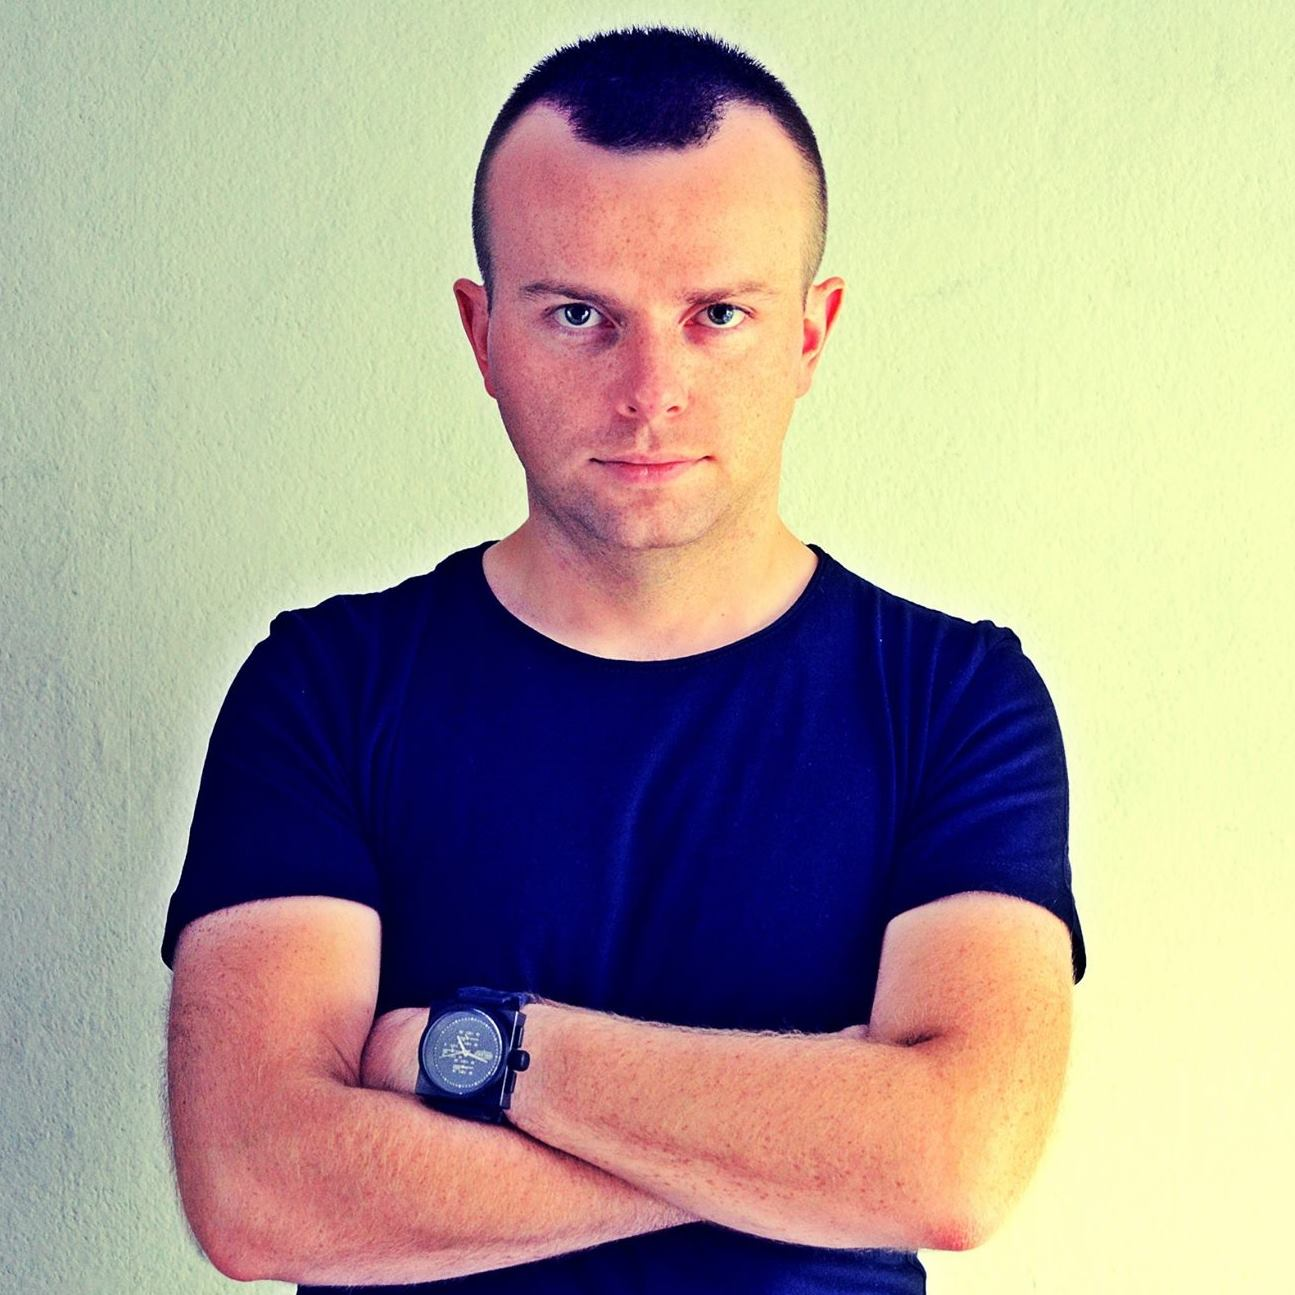
\includegraphics[width=2cm,keepaspectratio]{lbol.jpg} \\
      \hline
      From       & Essex, UK                                               & Lodz, Poland                                          \\
      Study      & MSc                                                     & BSc (3rd Year)                                        \\
      Society    & Mentor                                                  & Chair                                                 \\
      Speciality & AI                                                      & IoT                                                   \\
      University & (Past) Student Rep                                      & (Past) Student Rep                                    \\
                 & PAL Leader                                              & PAL Leader                                            \\
                 & Student Proctor                                         & Student Proctor                                       \\
      Work Exp   & Visteon                                                 & Self-employed DJ                                      \\
      \hline
    \end{tabular}
  \end{frame}
  \begin{frame}
    \frametitle{Previous Projects}
    \centering
    \begin{tabular}{p{4cm} p{4cm}}
      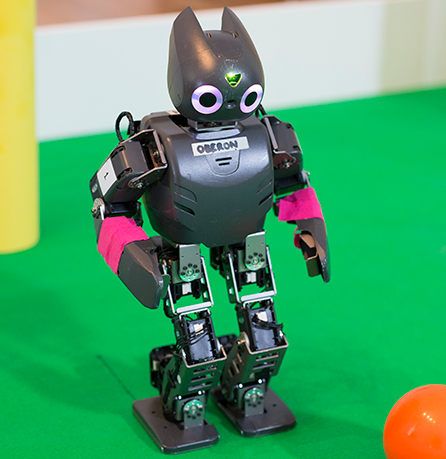
\includegraphics[width=2cm,keepaspectratio]{robocup.png}     &
      
\includegraphics[width=2cm,keepaspectratio]{netizens.png}   \\
      RoboCup - \emph{Football playing robots}                     &
      Netizens - \emph{UH hacking group}                          \\
      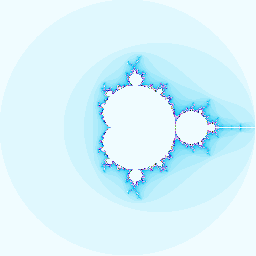
\includegraphics[width=2cm,keepaspectratio]{mandelbrot.png}  &
      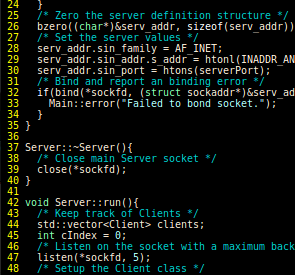
\includegraphics[width=2cm,keepaspectratio]{palproctor.png} \\
      General Programming - \emph{Too much to mention!}            &
      PAL \& Proctoring - \emph{Mentoring students}               \\
    \end{tabular}
  \end{frame}
  %%%%%%%%%%%%%%%%%%%%%%%%%%%%%%%%%%%%%
  % Aims
  %%%%%%%%%%%%%%%%%%%%%%%%%%%%%%%%%%%%%
  \section[Aims]{Aims}
  \begin{frame}
    \frametitle{Aims Over Time}
    \begin{itemize}
      \item \texttt{[ ]} Why are people hacking?
      \item \texttt{[ ]} What hacking is going on?
      \item \texttt{[ ]} Who is hacking?
    \end{itemize}
  \end{frame}
  \begin{frame}
    \frametitle{Aims Today}
    \begin{itemize}
      \item \texttt{[ ]} Learn about hacking
      \item \texttt{[ ]} Setup a development environment
      \item \texttt{[ ]} Introduction to the tools
      \item \texttt{[ ]} Build a monitoring program
    \end{itemize}
  \end{frame}
  %%%%%%%%%%%%%%%%%%%%%%%%%%%%%%%%%%%%%
  % History
  %%%%%%%%%%%%%%%%%%%%%%%%%%%%%%%%%%%%%
  \section[History]{History}
  \begin{frame}
    \frametitle{Why Hack?}
    \centering
    \begin{tabular}{c c}
      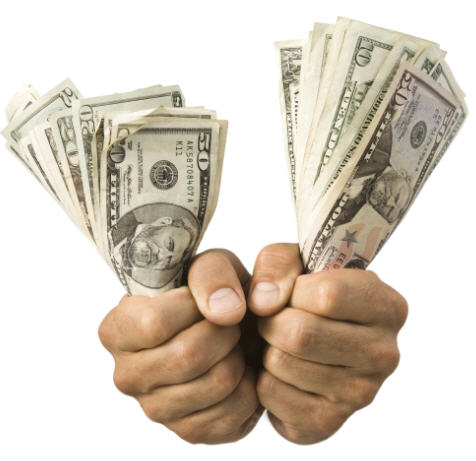
\includegraphics[height=2cm,keepaspectratio]{money.jpg}     &
      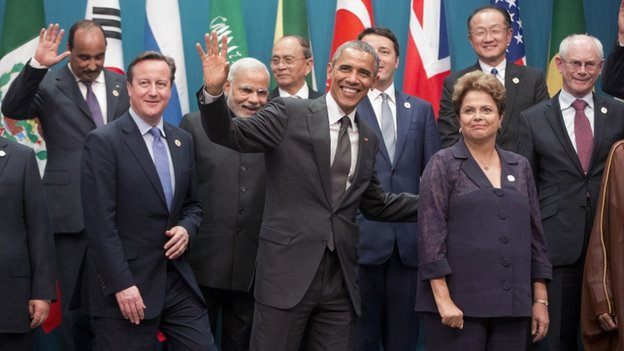
\includegraphics[height=2cm,keepaspectratio]{leaders.jpg}  \\
      Financial                                                   &
      Power                                                      \\
      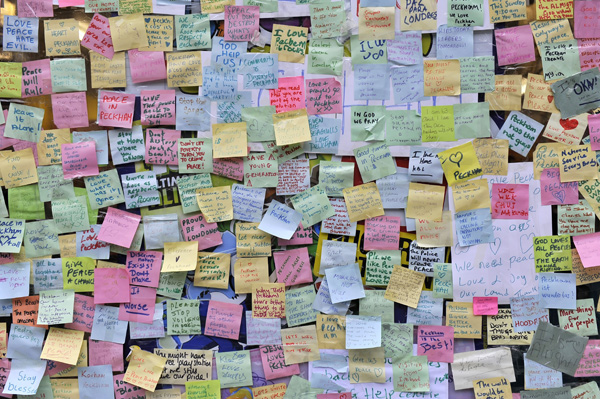
\includegraphics[height=2cm,keepaspectratio]{info.jpg}      &
      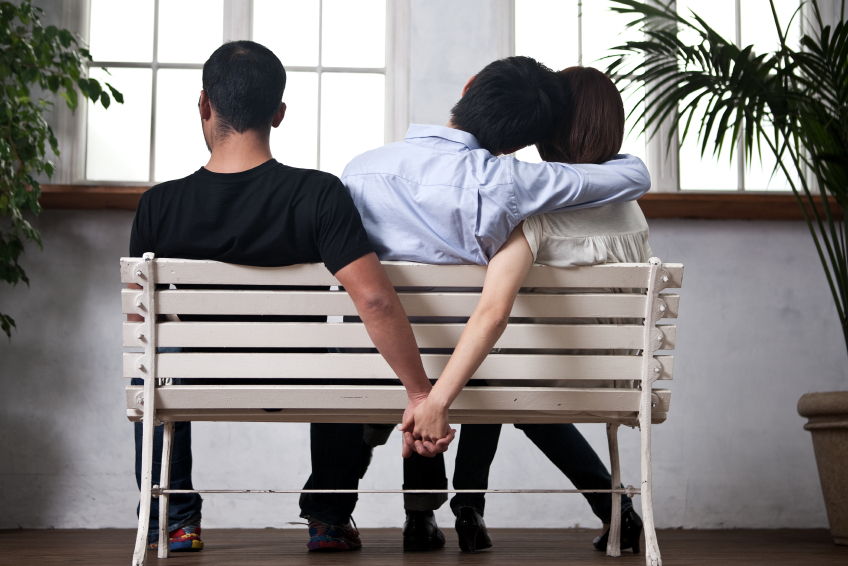
\includegraphics[height=2cm,keepaspectratio]{cheating.jpg} \\
      Information                                                 &
      Relationships                                              \\
    \end{tabular}
  \end{frame}
  \begin{frame}
    \frametitle{Targets of Hacking}
    \centering
    \begin{tabular}{c c}
      
\includegraphics[height=2cm,width=3cm,keepaspectratio]{dyn.png}        &
      
\includegraphics[height=2cm,width=3cm,keepaspectratio]{ovh.png}       \\
      DYN \cite{dyndns}                                                      &
      OVH \cite{ovhcld}                                                     \\
      
\includegraphics[height=2cm,width=3cm,keepaspectratio]{wikileaks.jpeg} &
      
\includegraphics[height=2cm,width=3cm,keepaspectratio]{janet.png}     \\
      WikiLeaks \cite{wiklks}                                                &
      JANET \cite{janisp}                                                   \\
    \end{tabular}
  \end{frame}
  \begin{frame}
    \frametitle{Attacks on Servers}
    \begin{itemize}
      \item (D)DoS - (Distributed) Denial of Service
      \item Privilege Escalation
      \item Database Injection
      \item Exploits (Metasploit and CVEs)
      \item And many, many others
    \end{itemize}
  \end{frame}
  %%%%%%%%%%%%%%%%%%%%%%%%%%%%%%%%%%%%%
  % Environment
  %%%%%%%%%%%%%%%%%%%%%%%%%%%%%%%%%%%%%
  \section[Env]{Environment}
  \begin{frame}
    \frametitle{Download}
    \begin{itemize}
      \item \url{https://www.virtualbox.org/wiki/Downloads}
      \item \url{http://coffeespace.org.uk/downloads/tiny-core-web-dev.zip}
      \item \url{http://coffeespace.org.uk/downloads/tiny-core-web-test.zip}
      \item \url{http://coffeespace.org.uk/downloads/Core-7.2.iso.zip}
    \end{itemize}
  \end{frame}
  \begin{frame}
    \frametitle{Virtual Machine}
    \textbf{TODO:} Write this section.
  \end{frame}
  \begin{frame}
    \frametitle{Running}
    \textbf{TODO:} Write this section.
  \end{frame}
  \begin{frame}
    \frametitle{Basics of Linux}
    \textbf{TODO:} Write this section.
  \end{frame}
  \begin{frame}
    \frametitle{Tools}
    \textbf{TODO:} Write this section.
  \end{frame}
  \begin{frame}
    \frametitle{Advanced}
    \textbf{TODO:} Discuss how to get more tools.
  \end{frame}
  %%%%%%%%%%%%%%%%%%%%%%%%%%%%%%%%%%%%%
  % Development
  %%%%%%%%%%%%%%%%%%%%%%%%%%%%%%%%%%%%%
  \section[Dev]{Development}
  \begin{frame}[fragile=singleslide]
    \frametitle{API}
    \begin{lstlisting}[caption=Java Hello World,language=Java]
/**
 * main()
 *
 * The main entry point into the program.
 *
 * @param args The arguments passed via the command line.
 **/
public static void main(String[] args){
  System.out.println("Hello World");
}
    \end{lstlisting}
  \end{frame}
  %%%%%%%%%%%%%%%%%%%%%%%%%%%%%%%%%%%%%
  % Conclusion
  %%%%%%%%%%%%%%%%%%%%%%%%%%%%%%%%%%%%%
  \section[End]{Conclusion}
  \begin{frame}
    \frametitle{Achievements}
    \textbf{TODO:} Write this text.
  \end{frame}
  \begin{frame}
    \frametitle{Wrapping Up}
    \begin{block}{}
      \centering
      Any questions?
    \end{block}
  \end{frame}
  \begin{frame}
    \frametitle{References}
    \begin{thebibliography}{}
      \bibitem{dyndns}
        Paganini, P.
        ``150,000 IoT Devices behind the 1Tbps DDoS attack on OVH",
        URL: \url{http://securityaffairs.co/wordpress/51726/cyber-crime/ovh-hit-botnet-iot.html?},
        2016.
      \bibitem{ovhcld}
        York, K.
        ``Dyn Statement on 10/21/2016 DDoS Attack",
        URL: \url{http://dyn.com/blog/dyn-statement-on-10212016-ddos-attack/},
        2016.
      \bibitem{wiklks}
        WikiLeaks.
        ``WikiLeaks",
        URL: \url{https://www.wikileaks.org/},
        2016.
      \bibitem{janisp}
        Martin, A.
        ``UK research network Janet under ongoing and persistent DDoS attack",
        URL: \url{http://www.theregister.co.uk/2015/12/07/janet_under_persistent_ddos_attack/},
        2016.
    \end{thebibliography}
  \end{frame}
\end{document}
